%!TeX root=../tese.tex
\chapter{Grau limitado}
\label{cap:grau-limitado}

% ---------------------------------------
% ------- Vibe coding começa aqui -------
% ---------------------------------------

% Comando personalizado para desenhar o grafo de Andrásfai com parâmetro d
\newcommand{\drawAndrasfai}[1]{%
  \def\d{#1}                              % parâmetro d
  \pgfmathsetmacro\n{int(3*\d - 1)}       % número de vértices n = 3d - 2
  \begin{tikzpicture}[scale=1.5,
    every node/.style={circle, draw, fill=white, inner sep=1pt, font=\small}]
  
  % 1. Coloca os vértices uniformemente em círculo
  \foreach \i in {0,...,\numexpr \n-1 \relax} {
    \pgfmathsetmacro\angle{90-360*\i/\n}
    \node (v\i) at (\angle:1) {\i};       % vértice v_i na posição angular correspondente
  }

  % 2. Para cada vértice, conecta aos d vértices mais distantes
  \foreach \i in {0,...,\numexpr \n-1 \relax} {
    \foreach \offset in {0,...,\numexpr \d-1 \relax} {
      \pgfmathsetmacro\j{mod(\i + \d + \offset, \n)} % vértice mais distante no ciclo
      \pgfmathtruncatemacro{\ii}{\i}
      \pgfmathtruncatemacro{\jj}{\j}
      \ifnum\ii<\jj
        \draw (v\ii) -- (v\jj);          % desenha aresta se ii < jj (para evitar duplicação)
      \fi
    }
  }

  \end{tikzpicture}
}

% --------------------------------------
% ------ Vibe coding termina aqui ------
% --------------------------------------

Vamos tentar resolver quando $\delta(G)$ é grande?
Ok, ok, você vai dizer ``mas o resultado do capítulo 2 já cobre isso''.
Verdade, mas queremos mais \textit{estrutura} sobre os conjuntos que geram $D(G)$, então ainda vale a pena estudar esses casos!

Seja $d \geq 1$ um inteiro positivo.

\begin{definition}
  Seja $d \geq 1$ um inteiro positivo.
  O \emph{grafo de Andrásfai} $F_d$ é o grafo com vértices $\{0,1,\dots,3d-2\}$ e arestas entre $i$ e $i+d+j$ para cada $j \in \{0,1,\dots,d-1\}$.
  Uma forma de representar os grafos de Andrásfai é colocar os vértices em uma circunferência em sentido horário como vértices de $(3d-1)$-ágono regular e ligar cada vértice com os $d$ vértices mais distantes dele.

  \begin{figure}[htbp]
    \centering

    \begin{subfigure}[b]{0.22\textwidth}
      \centering
      \drawAndrasfai{1}
      \caption*{$F_1$}
    \end{subfigure}
    \hfill
    \begin{subfigure}[b]{0.22\textwidth}
      \centering
      \drawAndrasfai{2}
      \caption*{$F_2$}
    \end{subfigure}
    \hfill
    \begin{subfigure}[b]{0.22\textwidth}
      \centering
      \drawAndrasfai{3}
      \caption*{$F_3$}
    \end{subfigure}
    \hfill
    \begin{subfigure}[b]{0.22\textwidth}
      \centering
      \drawAndrasfai{4}
      \caption*{$F_4$}
    \end{subfigure}

    \caption{Grafos de Andrásfai para $d = 1$ a $d = 4$. Observe que $F_d$ é $d$-regular e livre de triângulos.}
  \end{figure}
\end{definition}

\begin{theorem}
  Seja $G$ um grafo livre de triângulos com $n$ vértices e $d \in \{1,2,\dots,9\}$.
  Se $\delta(G) > \frac{d}{3d-1}$, então $G$ está contido em um blow-up de $F_{d-1}$.
\end{theorem}

\begin{theorem}
  Seja $G$ um grafo livre de triângulos aresta com $n$ vértices tal que $\delta(G) > \frac{10n}{29}$ ou $\delta(G) > \frac{n}{3}$ e $\chi(G) \leq 3$.
  Então existe um inteiro $d \geq 1$ tal que $G$ é subgrafo de um blow-up de $F_d$.
\end{theorem}

\renewcommand{\emptyset}{\varnothing}

\begin{lemma}
  Seja $G$ um grafo e suponha que existem $F_1,F_2,F_3,F_4,F_5 \subseteq E$ tais que:
  \begin{itemize}
    \item $F_i \cap F_j = \emptyset$ para todo $i \neq j$ com $i,j \in \{1,2,3,4,5\}$;
    \item $G-F_i$ é bipartido para cada $i \in \{1,2,3,4,5\}$.
  \end{itemize}
  Então $G$ satisfaz a Conjectura \ref{conj:make-bipartite}.
\end{lemma}

Esse Lema vai funcionar para $F_4$, mas não para $F_5$.

\begin{corollary}
  Se $\delta(G) > 4n/11$, então $D(G) \leq \frac{n^2}{25}$.
\end{corollary}

\begin{center}
  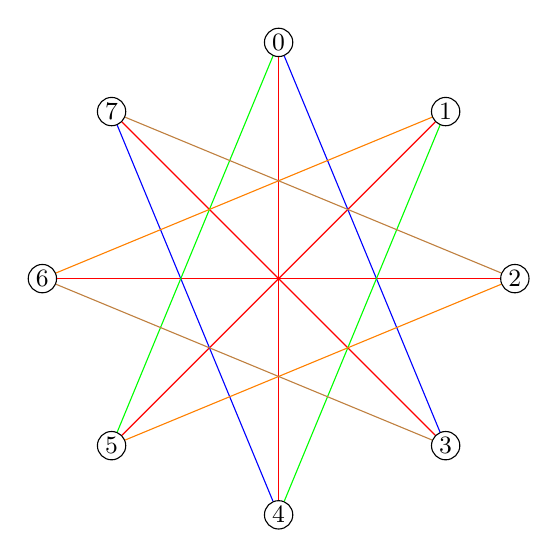
\begin{tikzpicture}[scale=3,
    every node/.style={circle, draw, fill=white, inner sep=1pt, font=\small}]
  
  % 1. Coloca os vértices uniformemente em círculo
  \foreach \i in {0,...,7} {
    \pgfmathsetmacro\angle{90-360*\i/8}
    \node (v\i) at (\angle:1) {\i};       % vértice v_i na posição angular correspondente
  }

  \draw [red] (v0)--(v4);
  \draw [red] (v1)--(v5);
  \draw [red] (v2)--(v6);
  \draw [red] (v3)--(v7);

  \draw [blue] (v0)--(v3);
  \draw [blue] (v7)--(v4);

  \draw [green] (v1)--(v4);
  \draw [green] (v0)--(v5);

  \draw [orange] (v1)--(v6);
  \draw [orange] (v2)--(v5);

  \draw [brown] (v3)--(v6);
  \draw [brown] (v2)--(v7);

  \end{tikzpicture}
\end{center}